\chapter{Implementation}
\label{sec:implementation}

\section{Lösungsansatz}
\label{sec:Lösung}

Übergeordnet lässt sich die Aufgabe dieser Arbeit damit zusammenfassen, aus einem Bild Wissen zu ziehen, welches einen hohen Grad an Abstraktion beinhaltet. Da herkömmliche Neuronale Netzwerke alleine nicht für diese Aufgabe ausreichen, wird in dieser Arbeit der Ansatz untersucht, durch die Kombination aus Neuronalem Nerz und semantischem Netzwerk ein System zu schaffen und zu bewerten, welches aus einem Bild Informationen über z.B. die Räumlichkeit und Handlungsfelder, theoretisch aber über jegliches Thema, abstrahieren kann. 


\begin{figure}[h]
	
	\begin{center}
		
		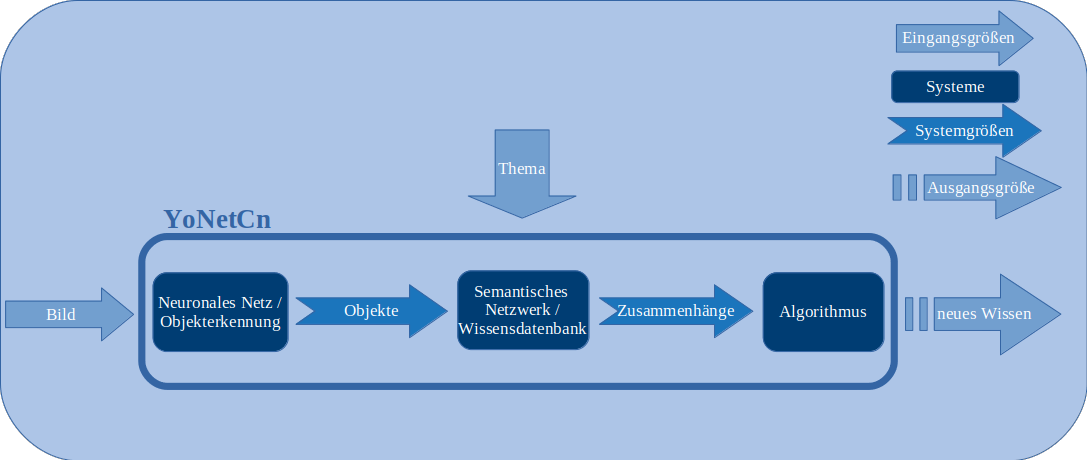
\includegraphics[width=14cm]{images/Masteridee.png}
		
		\caption{Aufbau System YoNetCn}
		
		\label{system_Bild}
		
	\end{center}
	
	
\end{figure}


In Abbildung X.x ist das Konzept für dieses System, welches unter dem Namen YoNetCn zusammengefasst wird, dargestellt. Die primäre Eingangsgröße für YoNetCn ist ein Bild,in welchem durch ein Neuronales Netz Objekte erkannt werden. Die Objekte dienen zusammen mit der sekundären Eingangsgröße, einem Thema oder Themengebiet, einem Semantischen Netz als Eingangsgrößen. Ausgegeben werden vom semantischem Netz als Systemgröße die Zusammenhänge zwischen den Objekten und dem Thema. Ein Algorithmus bewertet und filtert diese Zusammenhänge und schließt daraus auf neues Wissen. Als Beispiel hierfür dient die Szenenerkennung. 



\begin{figure}[h]
	
	\begin{center}
		
		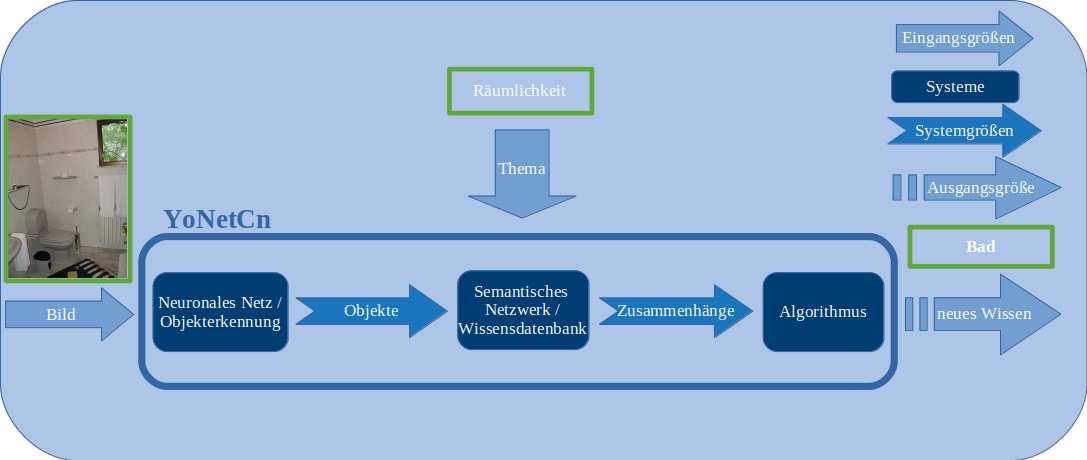
\includegraphics[width=14cm]{images/Masteridee_2.png}
		
		\caption{Szenenerkennung mit YoNetCn}
		
		\label{system_Bild}
		
	\end{center}
	
	
\end{figure}


Abbildung X.x zeigt die Szenenerkennung mit YoNetCn am Beispiel eines Bildes von einem Bad. Wird zu diesem Bild das Thema Räumlichkeit als sekundäre Eingangsgröße eingegeben, so wird als Ausgabe Bad ausgegeben. Bei gleichem Bild, jedoch mit sekundärer Eingabe Tätigkeit, soll YoNetCn Adjektive wie duschen, auf Toilette gehen, oder Zähne putzen ausgeben. Theoretisch sind jegliche sekundären Eingangsgrößen möglich, jedoch wurde sich in dieser Arbeit auf die Themen Räumlichkeit und Tätigkeit beschränkt, da der zeitliche Rahmen dieser Arbeit ansonsten gesprengt werden würde und diese beiden Themengebiete als Nachweis für die grundsätzliche Durchführbarkeit der Aufgabenstellung ausreichen. 


Auf Grundlage des konkreten Anwendungsbereiches von YoNetCn, der Servicerobotik, wurde als Stellgröße die Verarbeitungszeit und die Genauigkeit definiert. Ein Serviceroboter soll in Echtzeit erkennen können, welche Objekte sich in dem  Raum befinden, in welchem Raum er sich befindet und welche Handlungen mit den erkannten Objekten durchführbar sind. Da Echtzeit je nach Anwendungsbereich unterschiedlich ausgelegt wird, müssten für diesen Anwendungsfall genauere Untersuchungen für eine angemessene Reaktionszeit des Roboters durchgeführt werden, was jedoch nicht Umfang dieser Arbeit ist. Für YoNetCn wurde ein Wert von kleiner 10 Sekunden für die Reaktionszeit definiert, der Einfluss der Auslegung von YoNetCn auf die Reaktionszeit wird im Verlauf der Arbeit genauer beschrieben. 

Die Genauigkeit von YoNetCn wird am Beispiel der Räumlichkeit genauer untersucht und es werden verschiedene Stell- und Störgrößen, deren Einfluss auf die Genauigkeit herausgearbeitet.
Als Beispiel hat ein großes Neuronales Netz, welches sehr viele Objekte erkennt, einen positiven Einfluss auf die Genauigkeit, jedoch wird dadurch die Verarbeitungszeit negativ beeinflusst, da größere Netze mehr Rechenoperationen als kleine benötigen. Entsprechend gilt es eine Balance zwischen den beiden Stellgrößen zu finden. 
Semantische Netzwerke basieren auf Sprache. Da Sprache mehrdeutig sein kann und unter Umständen zu Missverständnissen führt, allgemein nicht immer klar definiert ist im Vergleich zur Informatik und Mathematik, wird auch das Zusammenspiel zwischen dem Neuronalen Netz und dem Semantischen Netz untersucht und entsprechende Störgrößen herausgearbeitet. 


Da YoNetCn speziell für die Servicerobotik entwickelt wurde, besteht der Anspruch einer Einbindung in ein verteiltes System. Darunter ist zu verstehen, dass mehrere Roboter auf die Funktion von YoNetCn zugreifen können, ebenso die Ergebnisse zentral zugänglich sind. Die Vision, welche hinter diesem Anspruch steht, ist, dass in einer Umgebung, zum Beispiel ein Altenheim, mehrere Roboter mit unterschiedlichen Fähigkeiten eingesetzt werden können. Einer dieser Roboter hat eine Kamera und kann Bilder empfangen und diese an YoNetCn weiterleiten. Aus den Bildern werden Aufgaben abgeleitet, wie z.B. einen Kaffee kochen, oder das Geschirr aus dem Büro holen und dieses in der Küche in die Spülmaschine einräumen. Der Roboter mit der Kamera hat jedoch keinen Greifarm, ein andere wiederum schon. Die Aufgaben werden Zentral gesteuert und an die Expertenroboter, die entsprechende Aufgaben bewältigen können, weitergeleitet. So entsteht eine Kollaboration zwischen den Robotern. 

Auch zwischen den Robotern und den Menschen in der Umgebung, soll ein Austausch stattfinden. So erkennt ein Roboter Beispielsweise eine schmutzige, leere Kaffeetasse im Büro. Diese Information mit dem Wissen, dass in der Küche eine Kaffeemaschine steht, ermöglicht es, die Aufgabe des Kaffeekochens anzubieten. Über eine App auf dem Smartphone werden die entsprechenden Service angezeigt und können vom Menschen ausgewählt oder priorisiert werden. 

Ergänzend zur definierten Aufgabe dieser Arbeit wird daher eine Schnittstelle zum Menschen entwickelt. 

\begin{figure}[h]
	
	\begin{center}
		
		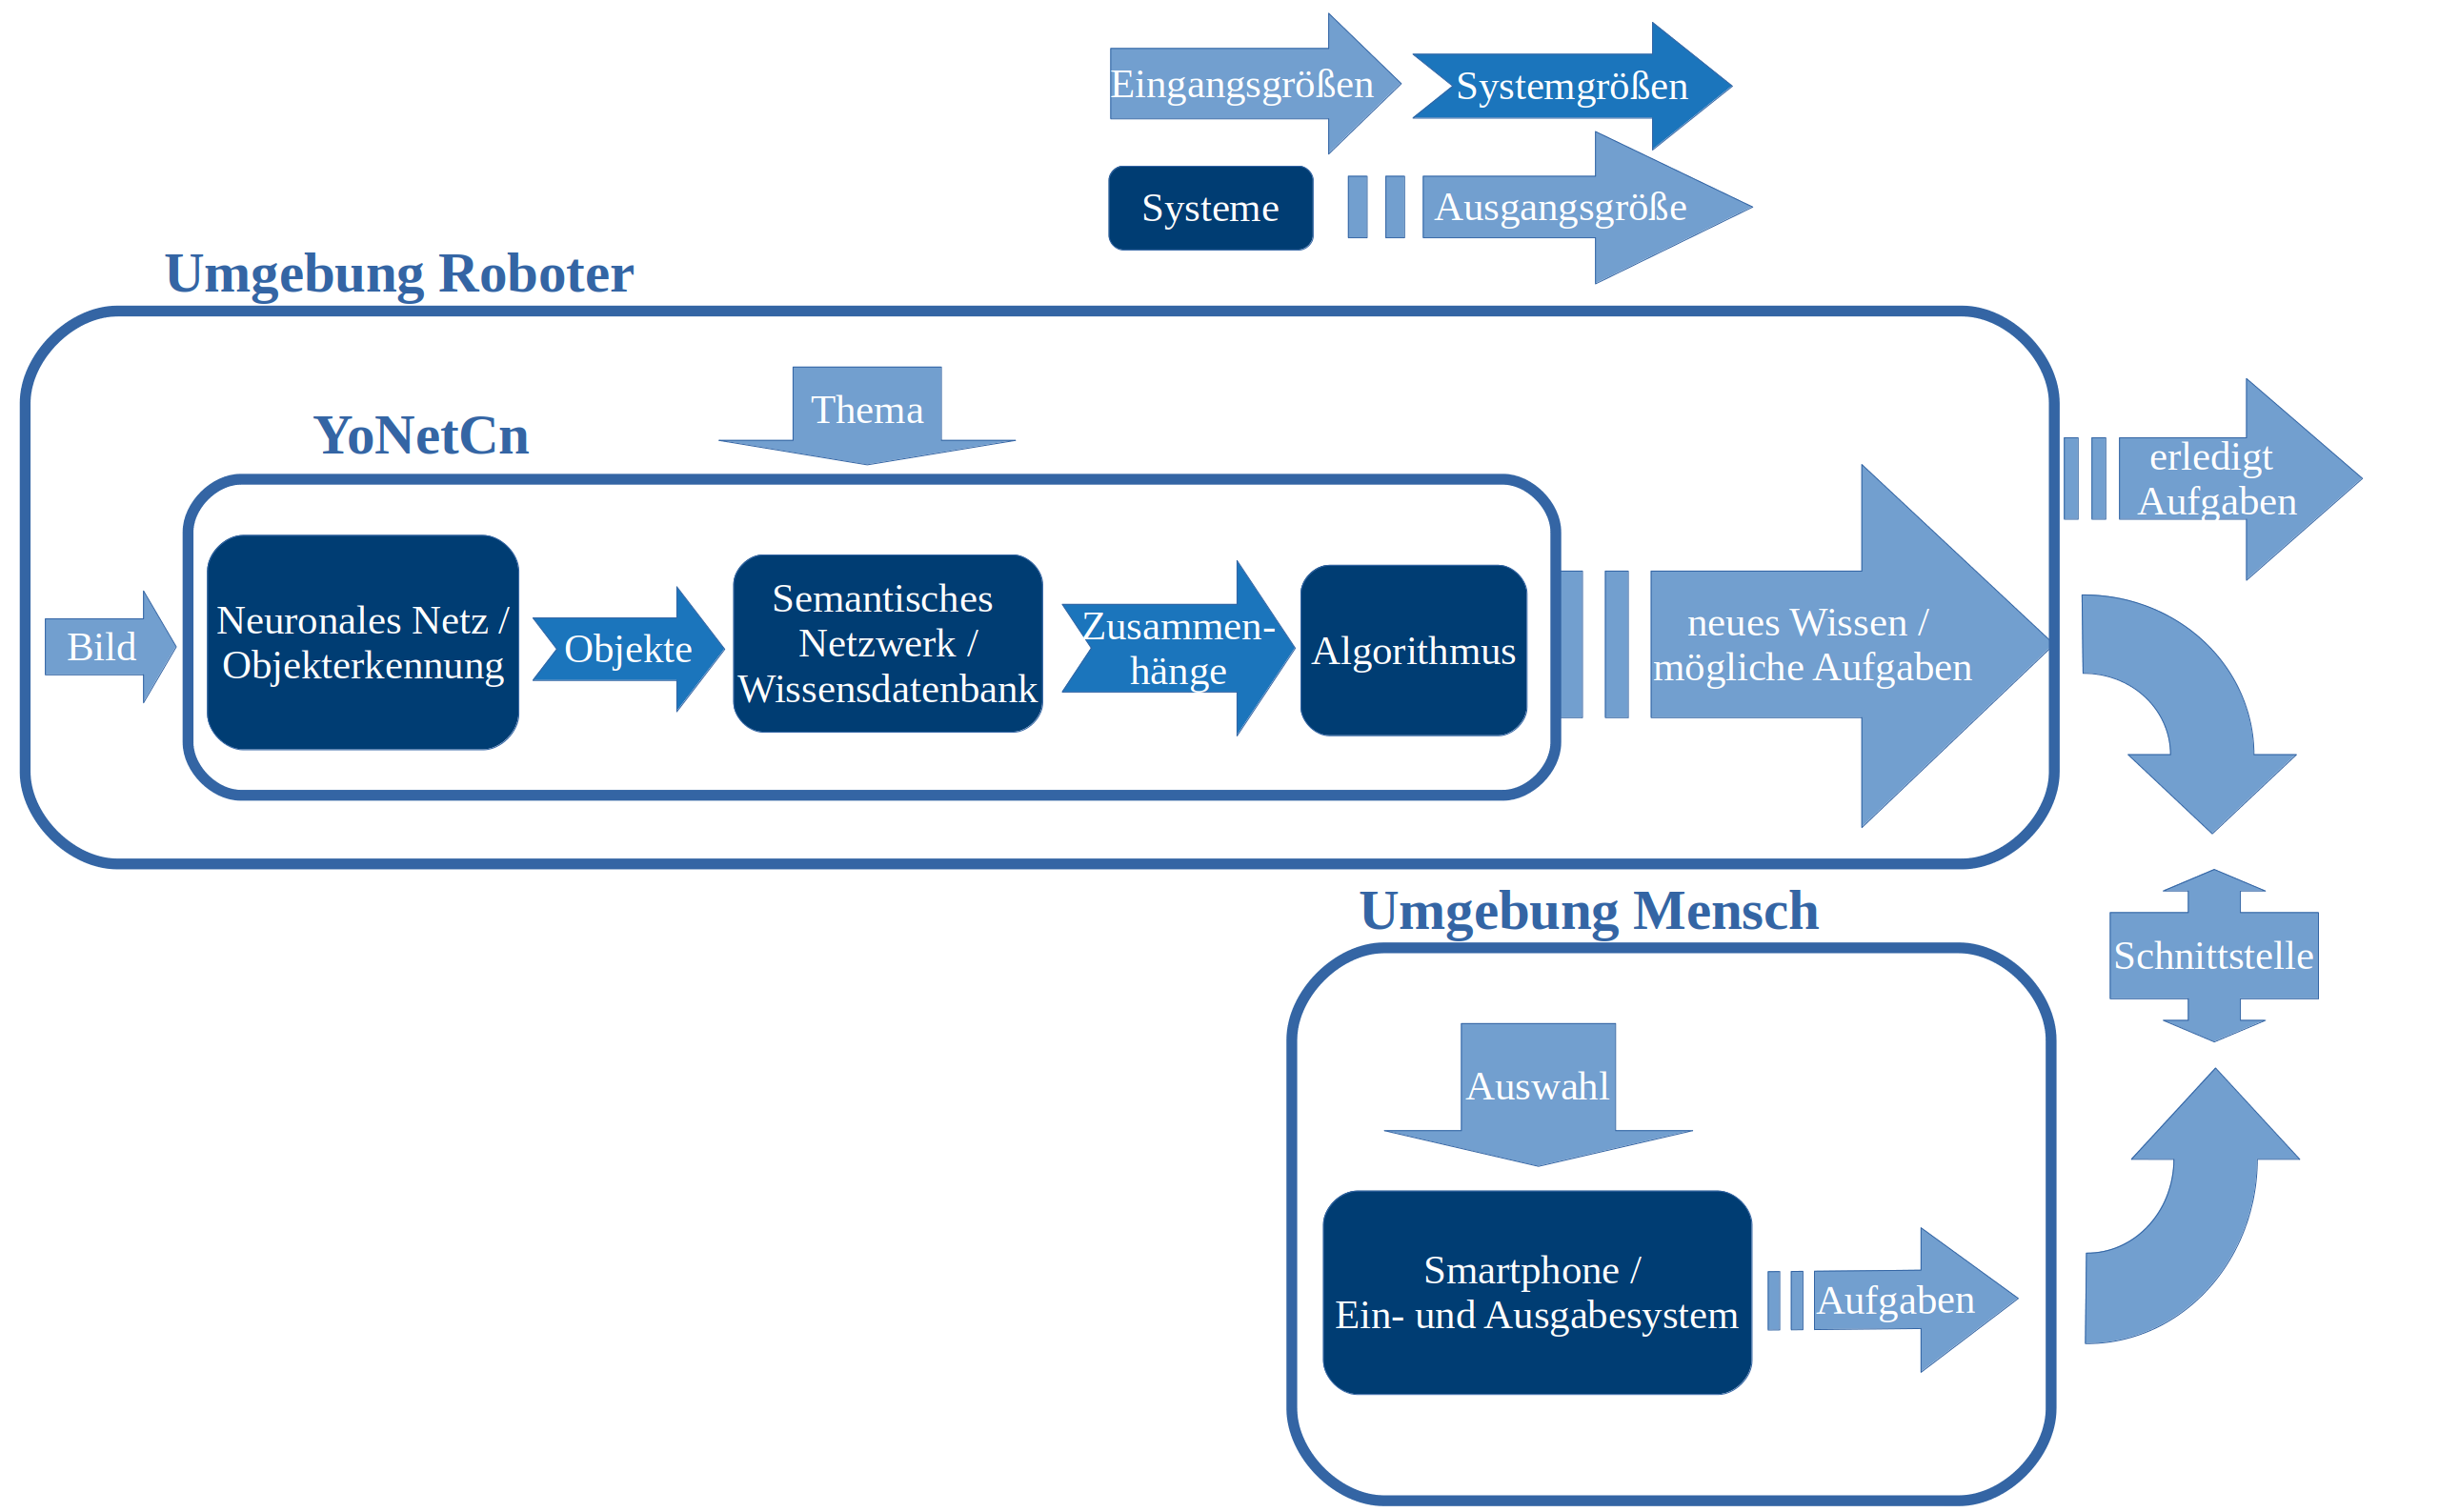
\includegraphics[width=16cm]{images/Masteridee_3.png}
		
		\caption{Roboter Mensch System}
		
		\label{Roboter_Mensch_System}
		
	\end{center}
	
	
\end{figure}


Abbildung X.x zeigt die erweiterte Aufgabenstellung, welche eine Schnittstelle zwischen der Umgebung Roboter und der Umgebung Mensch beinhaltet. 
Über die Rückmeldung durch den Menschen, könnte noch eine Lernfunktion für die Roboterumgebung integriert werden, sodass beispielsweise Aufgaben die öfters ausgewählt wurden, von YoNetCn bevorzugt angeboten werden. Auch wäre es denkbar dem Menschen nicht nur eine Auswahl von Aufgaben anzubieten, sondern, dass dieser neue Aufgaben definiert oder sogar den Robotern Aufgaben beibringt. 
Die Umsetzung der angebotenen Aufgaben ist nicht Teil dieser Arbeit, es werden lediglich potenzielle Aufgaben von YoNetCn ausgegeben und der Umgebung Mensch mitgeteilt. 





\section{Umsetzung}
\label{sec:umsetzung}





\begin{figure}[h]
	
	\begin{center}
		
		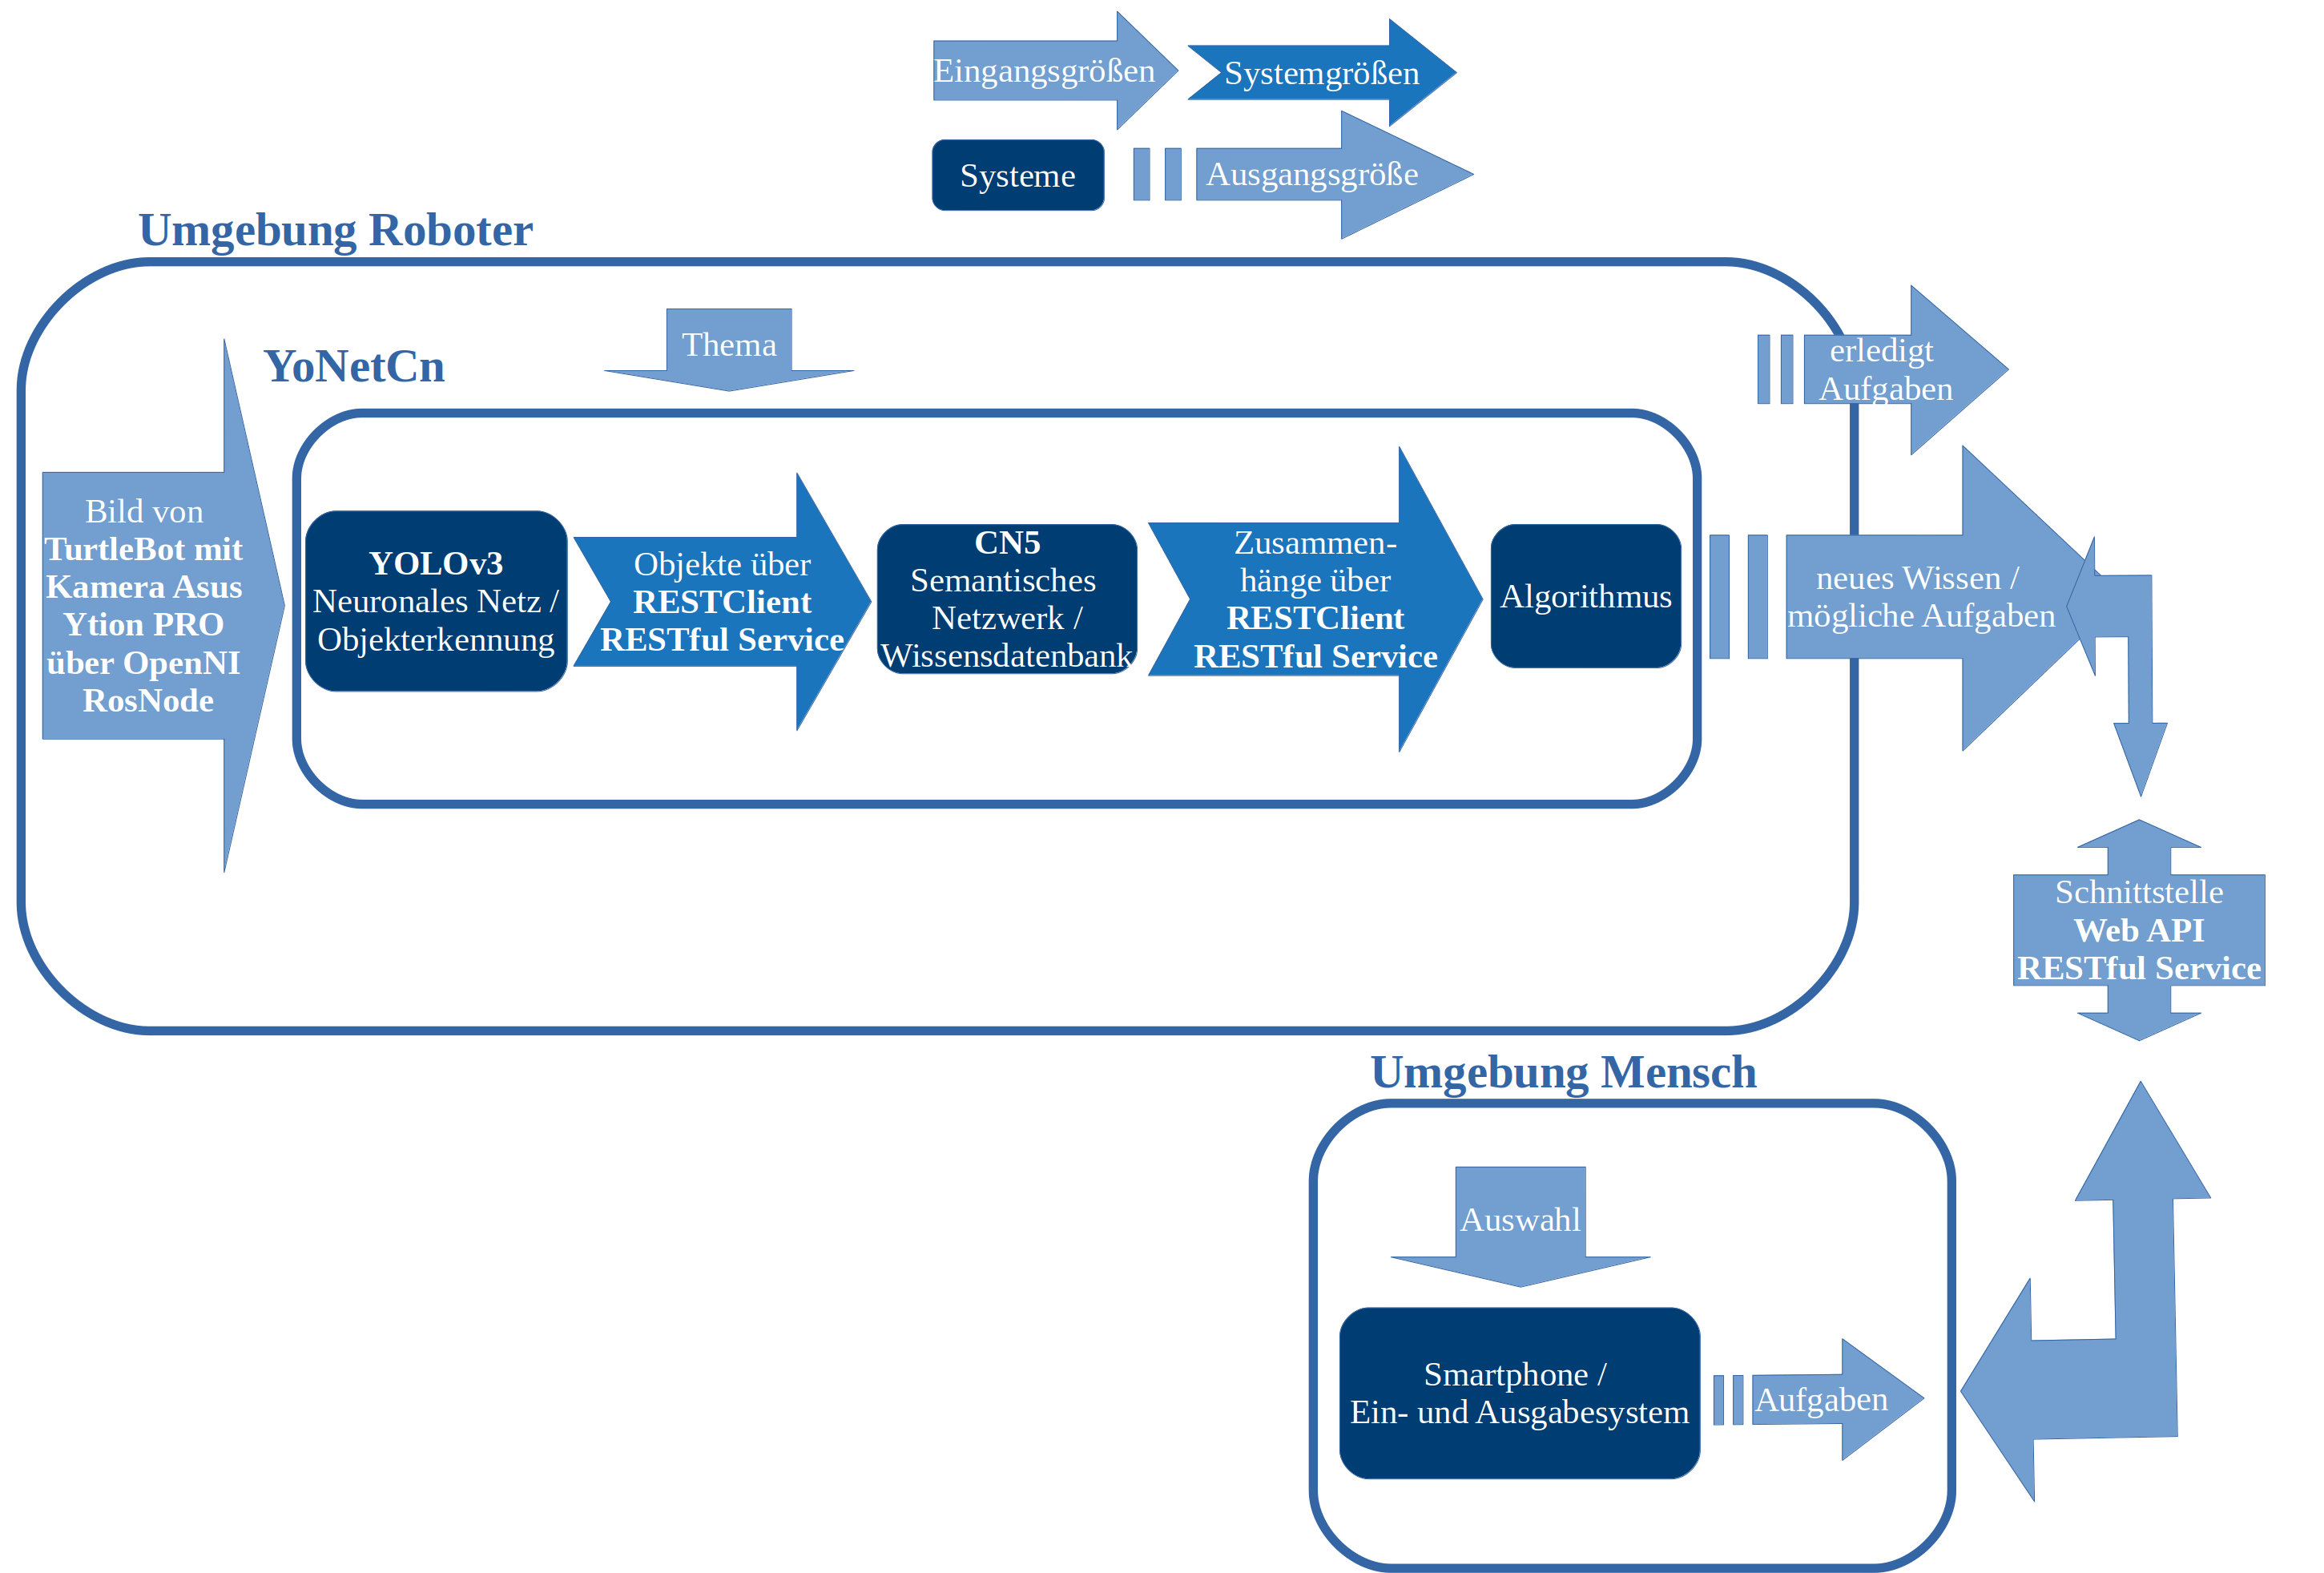
\includegraphics[width=16cm]{images/Masteridee_4.png}
		
		\caption{Roboter Mensch System}
		
		\label{Roboter_Mensch_System}
		
	\end{center}
	
	
\end{figure}


